\chapter*{Avant-propos}
\addcontentsline{toc}{chapter}{Avant-propos}
\markboth{AVANT-PROPOS}{}

\section*{Ce que vous allez comprendre}

Un utilisateur arrive sur un site web, crée un compte, choisit « Ubuntu, bureau
graphique, 30 minutes », clique. Quinze secondes plus tard il a une machine
Linux à lui, avec une adresse SSH, un terminal dans son navigateur et un bureau
XFCE complet. Trente minutes plus tard, la machine a disparu toute seule et le
port qu'elle occupait est rendu.

Derrière ce clic, il y a un serveur web, une base de données, un démon Docker
sur trois machines différentes, un ordonnanceur qui choisit laquelle, un
service qui surveille les horloges, des certificats, un pare-feu, un coffre à
secrets, et une chaîne d'intégration qui refuse de publier quoi que ce soit
tant que onze contrôles ne sont pas au vert.

Ce document explique chacune de ces pièces. Pas en survol : le code exact, les
raisons de chaque choix, et les erreurs commises en chemin.

\begin{retenir}
À la fin de ce guide, vous devez être capable de reconstruire un projet de ce
type sans le recopier. C'est pour cela que chaque chapitre explique d'abord
\emph{pourquoi} avant de montrer \emph{comment}.
\end{retenir}

\section*{À qui s'adresse ce guide}

À quelqu'un qui sait programmer un peu, qui a déjà vu une ligne de commande,
et qui n'a jamais construit d'infrastructure. Aucune connaissance préalable de
Docker, d'Ansible, de Vagrant, de Flask ou de la sécurité web n'est supposée.

Chaque notion nouvelle est introduite dans un encadré bleu avant d'être
utilisée. Les pièges réellement rencontrés sont signalés en orange. Les points
à retenir sont en vert.

\begin{notion}{Comment lire les extraits de code}
Les extraits sont tirés du dépôt réel, sans retouche. Quand un fichier est trop
long pour tenir ici, seules les lignes qui portent l'idée sont reproduites et
les coupures sont marquées. Le chemin du fichier est toujours donné : vous
pouvez ouvrir l'original pour voir le reste.
\end{notion}

\section*{Le résultat, en images}

Avant de plonger dans la mécanique, voici ce que l'utilisateur voit.

\begin{figure}[htbp]
\centering
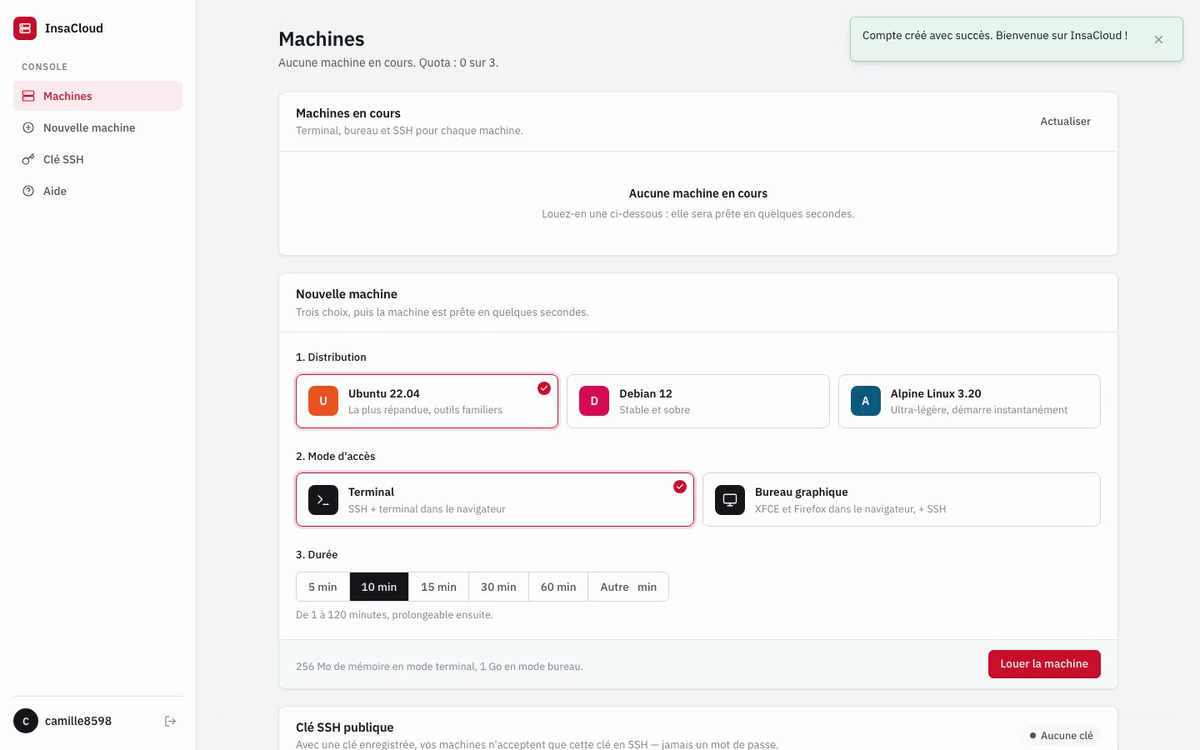
\includegraphics[width=0.78\textwidth]{../docs/03-tableau-de-bord.png}
\caption{Le tableau de bord. Les machines en cours, leur temps restant, et le
formulaire de location. Tout tient sur une page : c'est un choix, pas une
limite.}
\end{figure}

\begin{figure}[htbp]
\centering
\begin{minipage}{0.48\textwidth}
  \centering
  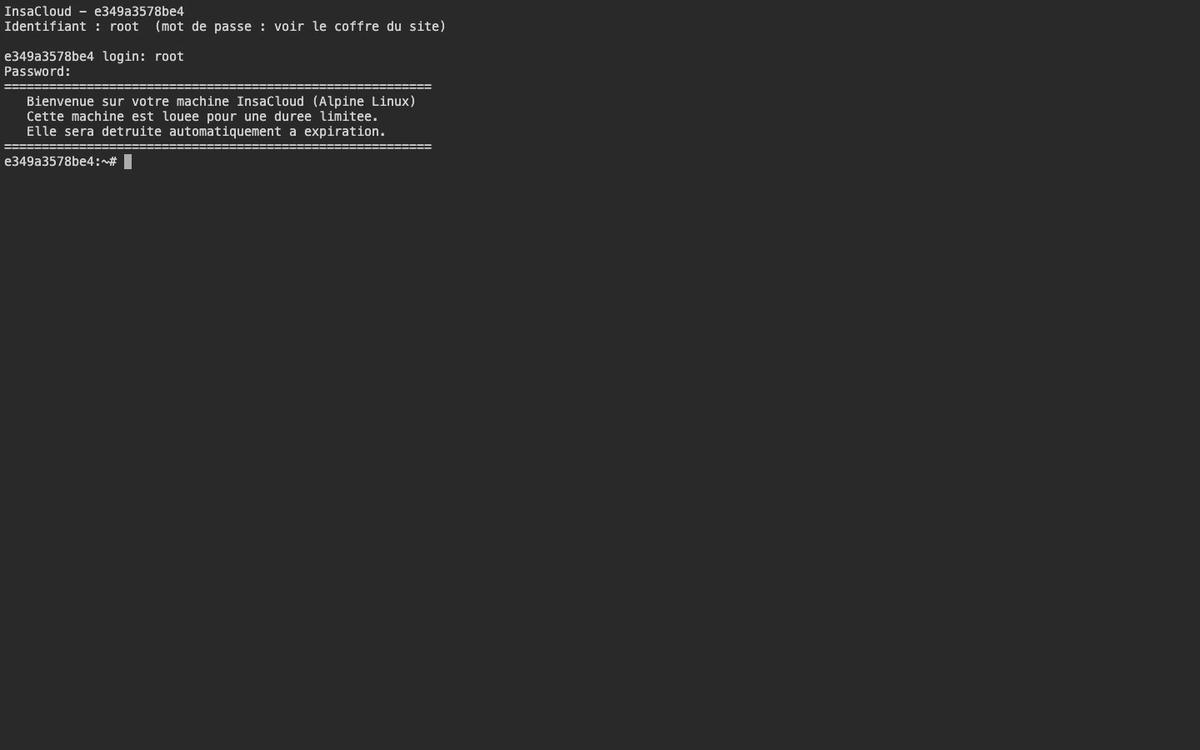
\includegraphics[width=\textwidth]{../docs/07-terminal-web.png}
\end{minipage}\hfill
\begin{minipage}{0.48\textwidth}
  \centering
  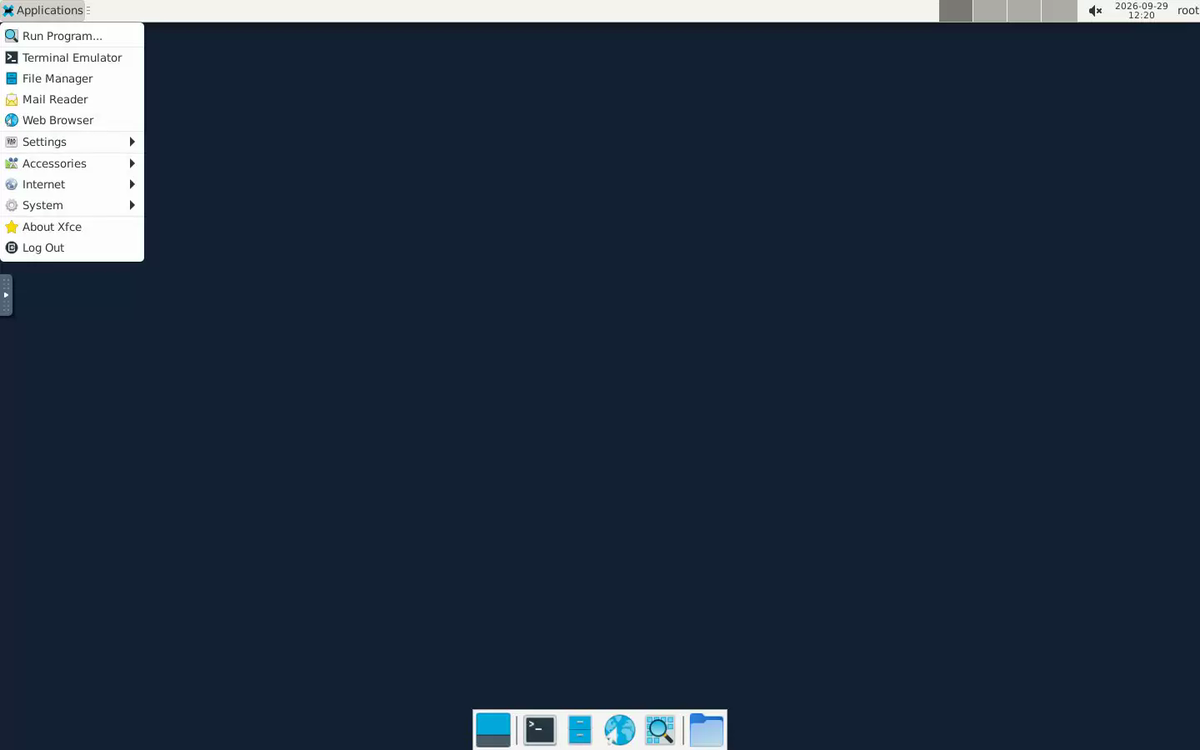
\includegraphics[width=\textwidth]{../docs/09-bureau-applications.png}
\end{minipage}
\caption{À gauche, un terminal dans le navigateur, sans rien installer. À
droite, un bureau XFCE complet avec Firefox, également dans le navigateur. La
même machine peut offrir l'un ou l'autre selon le mode choisi à la location.}
\end{figure}

\section*{Comment ce guide est organisé}

\begin{description}
\item[Partie I — Les notions] Ce qu'il faut savoir avant d'ouvrir le code :
  virtualisation, conteneurs, modèle web, infrastructure décrite en fichiers,
  et ce que « DevSecOps » veut dire concrètement.
\item[Partie II — L'architecture] La carte du territoire : qui parle à qui, où
  vivent les données, comment une machine naît et meurt.
\item[Partie III — La construction] Le cœur du guide. Chaque composant, son
  code, et les décisions qui l'ont façonné.
\item[Partie IV — Le déploiement] Comment tout cela arrive sur de vraies
  machines, en une commande, de façon reproductible.
\item[Partie V — La vérification] Les tests, la chaîne d'intégration, et le
  récit des défauts trouvés en faisant tourner le projet plutôt qu'en le
  relisant.
\item[Annexes] Commandes utiles, glossaire, erreurs fréquentes, et la grille de
  conformité au cahier des charges.
\end{description}

\section*{Le dépôt}

Tout le code commenté ici est public :
\url{https://github.com/aziz3r/insacloud}. Les chemins de fichiers mentionnés
dans le guide sont relatifs à la racine du dépôt.

\begin{center}
\begin{tabular}{@{}lr@{}}
\toprule
\textbf{Composant} & \textbf{Lignes} \\
\midrule
Application Flask (\fichier{2\_webapp/}) & environ 3\,500 \\
Tests (\fichier{2\_webapp/tests/}) & environ 1\,600 \\
Automatisation Ansible (\fichier{3\_ansible/}) & environ 1\,900 \\
Chaîne d'intégration (\fichier{.github/workflows/ci.yml}) & 601 \\
Images des machines (\fichier{1\_docker/}) & environ 400 \\
Infrastructure (\fichier{Vagrantfile}, \fichier{docker-compose.yml}) & 333 \\
\midrule
\textbf{Total} & \textbf{environ 10\,700} \\
\bottomrule
\end{tabular}
\end{center}
